\documentclass[main]{subfiles}
\begin{document}

%@@@@@@@@@@@@@@@@@@@@@@@@@@@@@@
% Main Topics: revised simplex algorithm and degeneracy and anti-cycling rules
% The Simplex Algorithm III - 23.10.2017
% author: Vanessa Leite

\section{Simplex Algorithm III}

\subsection{The worst-case running time of a simplex algorithm}
Assumption: we select a pivot-column $j \in N$ with the maximal absolute value
of reduced cost.

\paragraph{Theorem: Klee-Minty Cube (KMC)} Under the previous assumption, the
simplex algorithm can take "exponentially" (related with the input size) many
steps.

\subparagraph{Proof (construction/deformation of the cube): }

$\mathcal{P} = \{x \in \mathbb{R}^n \mid Ax \leq b \}$ is a deformation of the
cube.

\begin{figure}[!h]
  \label{fig:projection}
  \caption{Cube degeneracy: skip one vertice. It can be seen as a "cube", but
  the skipped vertex is not part of the problem.}
  \centering
    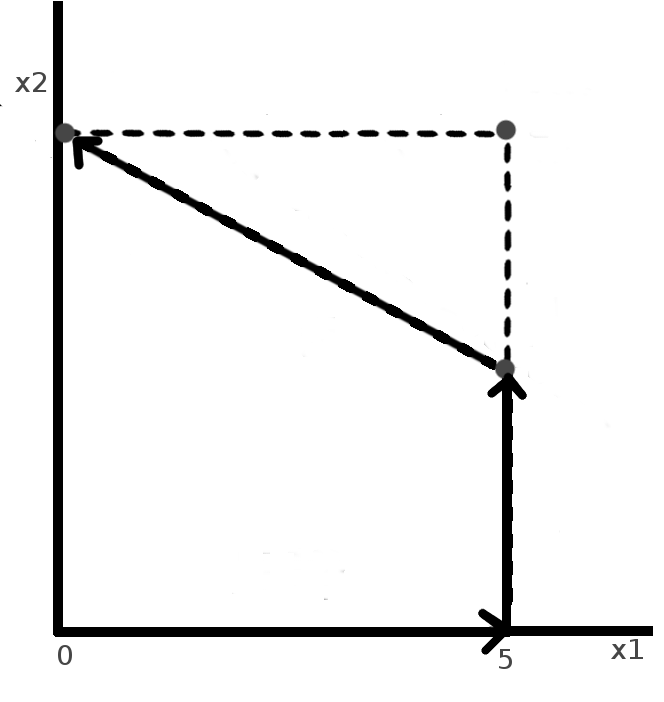
\includegraphics[width=0.2\textwidth]{imgs/kmc.png}
\end{figure}

\begin{equation*}
\begin{aligned}
& \max
& & 2x_1 + x_2 \\
& \text{subject to}
& & x_{1} \leq 5 \\
&&& 4x_1 + x_2 \leq 25\\
&&& x_1, x_2 \geq 0
\end{aligned}
\end{equation*}

\end{document}